\documentclass{article}

\usepackage[a4paper, left=2cm, right=2cm, top=3cm, bottom=2cm]{geometry}
\usepackage{amsmath}
\usepackage{mathptmx}
\usepackage{amsfonts}
\usepackage{amssymb}
\usepackage{dsfont}
\usepackage{amstext}
\usepackage{array}
\usepackage{lmodern}
\usepackage{arydshln}
\usepackage{rotating}
\usepackage{mathtools}
\usepackage{listings}
\usepackage{algorithm}
\usepackage{algpseudocode}
\usepackage{tikz}

\usetikzlibrary{arrows.meta, positioning, fit}

\usepackage{hyperref}
\hypersetup{
    colorlinks=true,
    linkcolor=black,
    citecolor=black,
    urlcolor=blue,
    pdfborder={0 0 0}
}

\setlength{\parindent}{0pt}
\setlength{\parskip}{6pt}

\usepackage[backend=bibtex]{biblatex}
\addbibresource{references.bib}

\usepackage{theorem}
\theoremheaderfont{\normalfont \bfseries}
\theorembodyfont{\it}
\newenvironment{proof}{\par\vspace*{1em}\noindent\textbf{Proof:}\par}{\par\hfill $\Box$\par}
\newtheorem{definition}{\textbf{Definition}}[section]
\newtheorem{theorem}{\textbf{Theorem}}[section]
\newtheorem{lemma}{\textbf{Lemma}}[section]
\newtheorem{example}{\textbf{Example}}[section]
\newtheorem{assumption}{\textbf{Assumption}}[section]
\newtheorem{proposition}{\textbf{Proposition}}[section]
\newtheorem{corollary}{\textbf{Corollary}}[section]
\newtheorem{remark}{\textbf{Remark}}[section]

\begin{document}

\begin{titlepage}

\begin{center}

\Huge Supplementary Materials for

\bfseries Title name

\bigskip
\bigskip

\Large 
Author name1

Author name2

\end{center}

\end{titlepage}

\tableofcontents
\newpage

\section{Preliminary on proximal standardization formulas}

\begin{figure}[ht]
    \centering
    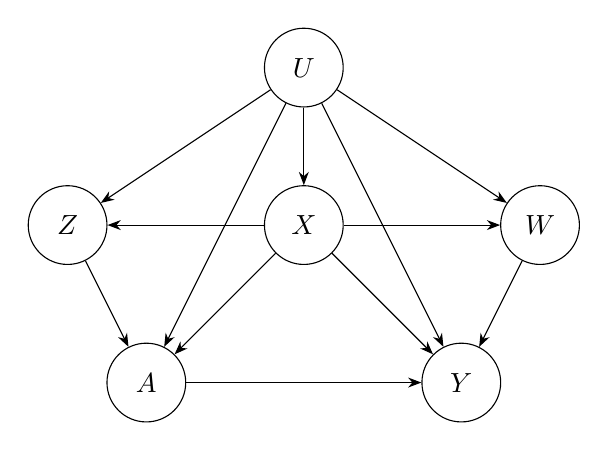
\begin{tikzpicture}[
        every node/.style={draw, circle, minimum size=1cm},
        every path/.style={->, >=Stealth}
    ]
    % Define nodes
    \node (U) at (3,5) {$U$};
    \node (X) at (3,3) {$X$};
    \node (Z) at (0,3) {$Z$};
    \node (W) at (6,3) {$W$};
    \node (A) at (1,1) {$A$};
    \node (Y) at (5,1) {$Y$};
    % Draw edges
    \draw (U) -- (X);
    \draw (U) -- (Z);
    \draw (U) -- (W);
    \draw (U) -- (A);
    \draw (U) -- (Y);
    \draw (X) -- (Z);
    \draw (X) -- (W);
    \draw (X) -- (A);
    \draw (X) -- (Y);
    \draw (A) -- (Y);
    \draw (Z) -- (A);
    \draw (W) -- (Y);
    \end{tikzpicture}
    \caption{\centering A DAG for proximal counterfactual model}
    \label{fig: pre_dagprox}
\end{figure}

Standardization in proximal causal framework is closely related to the proxy variables by the existence of the unobservable confounders. 
There are two classes of proxies. 
For those connecting both unobservable confounders and outcome, we call them outcome confounding proxies represented by $W$ in Figure \ref{fig: pre_dagprox}, 
while variables lying in between the treatment and unobservable confounders are treatment confounding proxies which is the node $Z$. 
Miao et al.\cite{WMiao2018} put forward a standardization formula using the outcome confounding proxies 
and Cui et al.\cite{YFCui2023} managed to identify the ATE with the treatment confounding proxies. 
Their identification methods require solving functions from Fredholm integral equations of the first kind. 
The solutions are called bridge functions because 
they remove the influence from the unobservable confounders 
and make it possible to identify ATE only with the observed. 
Moreover, the standardization formulas also depend on the completeness assumption on the distribution families of the confounder variables. 
We restate the important assumptions proposed by the pioneers in proximal causal inference as baseline for the later derivations.

\begin{assumption}(\textbf{Outcome confounding standardization formula}\cite{WMiao2018})
    
    \label{ass: pre_outcomehold}
    \begin{enumerate}
        \item \textbf{Completeness}: The distribution family for confounder variables $U,Z,A,X$ satisfies that 
                for any square-integrable function $g$ and for any $a$, $x$, $E[g(U)|Z, A = a, X = x] = 0$ almost surely if and only if $g(U) = 0$ almost surely. 
        \item \textbf{Existence of outcome confounding bridge function}: Denote the singular system of the conditional expectation operator $T: L_2(P_{(W,A,X)})\mapsto L_2(P_{(Z,A,X)})$ by $(\sigma_i, u_i, v_i)_{i\geq 1}$. 
                Then Picard's condition $\sum_{i\geq 1}\frac{|\left\langle E[Y|Z,A=a,X], v_i\right\rangle|^2}{\sigma^2_i}<\infty$ holds to make 
                integral equation
                \begin{equation}
                    \label{eq: pre_outbridge}
                    E[Y|Z,A=a,X] = \int h_a(w,A,X)dF(w|Z,A=a,X) = E[h_a(W,a,X)|Z,A=a,X], 
                \end{equation}
                solvable. 
    \end{enumerate}
\end{assumption}

\begin{assumption}(\textbf{Treatment confounding standardization formula}\cite{YFCui2023})

    \label{ass: pre_treatmenthold}
    \begin{enumerate}
        \item \textbf{Completeness}: The distribution family for confounder variables $U,W,A,X$ satisfies that 
                for any square-integrable function $g$ and for any $a$, $x$, $E[g(U)|W, A = a, X = x] = 0$ almost surely if and only if $g(U) = 0$ almost surely.
        \item \textbf{Existence of treatment confounding bridge function}: Denote the singular system of the conditional expectation operator $T^*: L_2(P_{(Z,A,X)})\mapsto L_2(P_{(W,A,X)})$ by $(\sigma^*_i, u^*_i, v^*_i)_{i\geq 1}$. 
                Then Picard's condition $\sum_{i\geq 1}\frac{|\left\langle \frac{1}{f(a|W,X)},v^*_i\right\rangle|^2}{(\sigma^*_i)^2}<\infty$ holds to make 
                integral equation solvable
                \begin{equation}
                    \label{eq: pre_treatbridge}
                    \frac{1}{f(a|W,X)} = \int q_a(z,A,X)dF(z|W,A=a,X) = E[q_a(Z,a,X)|W,A=a,X],
                \end{equation}
                where $f(a|W,X)=Pr\left\{A=a|W,X\right\}$.
    \end{enumerate}
\end{assumption}

If Assumptions \ref{ass: pre_outcomehold} and \ref{ass: pre_treatmenthold} hold, then we have the two standardization formulas, 
\begin{align*}
    E[Y^a] &= E[h_a(W,a,X)], \\
    E[Y^a] &= E[Yq_a(Z,a,X)\mathbb{1}_{A=a}].
\end{align*}
for all categories of $a$.

\section{Kernel embedded ATE estimator}

To estimate ATE in proximal causal framework, we adopt the dual kernel embedding method 
which was proposed by Dai et al.\cite{dai2017learning} to address the problem of learning from conditional distributions. 
These problems can be viewed as solving for functions that link conditional distributions to target values. 
Through a series of reformulations, including ERM reformulation, minimax problem reformulation through Fenchel duality and interchange of minimization and integration, 
and finally the kernel embeddings of means and cross-covariances, 
the method transforms the conditional expectation equation into a minimax problem for kernel embeddings of mean and (cross-)covariance. 
The method is based on the definition of the universal kernel\cite{steinwart2001influence}, 
whereby any bounded continuous function can be well approximated by functions belonging to the reproducing kernel Hilbert space (RKHS) induced by a universal kernel. 
Consequently, the solution obtained via kernel embedding can approximate the original bounded continuous function arbitrarily well.

Following Dai et al., 
Muandet et al.\cite{muandet2020dualinstrumentalvariableregression} applied the dual kernel embedding method to instrumental variable problems and 
obtained a closed-form solution in RKHS to approximate the causal functions in instrumental variable regression. 
Given the similarity between the integral equation for establishing the existence of bridge functions and instrumental variable regression, 
we apply the dual kernel embedding method to approximate the true boundedly continuous bridge functions $q_a$ and $h_a$ on RKHSs. 
And then to estimate ATE by plugging estimated bridge functions in the empirical form of the doubly robust standardization formula\cite{YFCui2023} 
\begin{equation*}
    \chi_{PDR} = E[\mathbb{1}_{A=1}q_1(Z,1,X)[Y-h_1(W,1,X)] - \mathbb{1}_{A=0}q_0(Z,0,X)[Y-h_0(W,0,X)] + h_1(W, 1, X)-h_0(W,0,X)].
\end{equation*} 

We start by giving a detailed derivation of finding the closed-form kernel embedded approximator $q^*_a$ on a RKHS of $q_a$ and its empirical form $\widehat{q}^*_a$. 
Then derive $h^*_a$ and $\widehat{h}^*_a$ with the simplest description.

\subsection{Tikhonov regularized kernel embedded treatment confounding bridge function}

The dual kernel embedding method relies on the original integral equation (\ref{eq: pre_treatbridge}), 
however which contains unknown propensity score $f(a|W,X)$. 
We give the equivalent form of this hard-to-tackle problem by tower property of conditional expectation. 
\begin{align}
    \label{eq: est_newintegral}
    \frac{1}{f(a|W,X)} &= E[q_a(Z,a,X)|W,A=a,X] \notag\\
    1 &= E[q_a(Z,a,X)|W,A=a,X]f(a|W,X) \notag\\
    1 &= E_A[E_Z[\mathbb{1}_{A=a}q_a(Z,a,X)|W,A,X]|W,X] \notag\\
    1 &= E_{ZA}[\mathbb{1}_{A=a}q_a(Z,a,X)|W,X]. 
\end{align}

Then we perform the ERM reformulation of (\ref{eq: est_newintegral}).
\begin{lemma}(\textbf{ERM reformulation})
    
    The true solution $q_a^{\star}(Z,a,X)$ for integral equation (\ref{eq: est_newintegral}) solves  
    the expected risk minimization problem with square loss for 1-dim data $l(x,y)=\frac{1}{2}(x-y)^2$ 
    \begin{equation}
        \label{eq: est_ERMreform}
        \min_{q_a\in L_2(P_{(Z,X|W,X)})} E_{W,X}[l(1, E_{ZA}[\mathbb{1}_{A=a}q_a(Z,a,X)|W,X])]. 
    \end{equation}
\end{lemma}
\begin{proof}
    First we consider the solution of $E_{W,X}[\frac{1}{2}(1-S(W,X))^2]$.
    For all $S\in L_2(P_{(W,X)})$, 
    since $E_{W,X}[\frac{1}{2}(1-S(W,X))^2]\geq0$ and it reaches the minimum 0 within a function class $\{S: E[S(W,X)]=1\}\subseteq L_2(P_{(W,X)})$,   
    it is clear that $E_Z[\mathbb{1}_{A=a}q_a^{\star}(Z,a,X)|W,X]\in\{S: E[S(W,X)]=1\}$ by Equation (\ref{eq: est_newintegral}). 
    Hence the true solution $q_a^{\star}(Z,a,X)$ for integral equation (\ref{eq: est_newintegral}) solves the ERM problem. 
\end{proof}

Next comes the minimax problem reformulation of ERM form. 

\begin{lemma}(\textbf{Minimax problem reformulation})
    
    The ERM form (\ref{eq: est_ERMreform}) of integral equation (\ref{eq: est_newintegral}) is equivalent to a 
    minimax problem 
    \begin{equation}
        \label{eq: est_saddlereform}
        \min_{q_a\in L_2(P_{(Z,X|W,X)})} \max_{u(\cdot,\cdot)\in\mathcal{M}(W,X)} E_{Z,W,A,X}[(\mathbb{1}_{A=a}q_a(Z,a,X)-1)u(W,X)]-\frac{1}{2}E_{W,X}[u^2(W,X)], 
    \end{equation} 
    where $\mathcal{M}(W,X)$ is the space of all measurable functions from $\mathcal{W}\times\mathcal{X}\mapsto\mathbb{R}$. 
\end{lemma}
\begin{proof}
    For simplicity, we denote the square loss function $l(x,y)$ by $l_x(y)$. 
    Its convex conjugate function is defined as $l_x^*(y):=\max_{u\in\mathbb{R}}\{uy-l_x(u)\}$.
    \begin{align}
         & \min_{q_a\in L_2(P_{(Z,X|W,X)})} E_{W,X}[l_1(E_{ZA}[\mathbb{1}_{A=a}q_a(Z,a,X)|W,X])] \notag\\
        =& \min_{q_a\in L_2(P_{(Z,X|W,X)})} E_{W,X}[\max_{u\in\mathbb{R}}\left\{uE_{ZA}[\mathbb{1}_{A=a}q_a(Z,a,X)|W,X]-l^*_1(u)\right\}] \notag\\                                                   
        =& \min_{q_a\in L_2(P_{(Z,X|W,X)})} E_{W,X}[\max_{u\in\mathbb{R}}\left\{uE_{ZA}[\mathbb{1}_{A=a}q_a(Z,a,X)|W,X]-u-\frac{1}{2}u^2\right\}] \label{eq: est_saddlereform1}\\
        =& \min_{q_a\in L_2(P_{(Z,X|W,X)})} \max_{u(\cdot,\cdot)\in\mathcal{M}(W,X)} E_{W,X}[u(W,X)E_{ZA}[\mathbb{1}_{A=a}q_a(Z,a,X)|W,X]-u(W,X)-\frac{1}{2}u^2(W,X)] \label{eq: est_saddlereform2}\\
        =& \min_{q_a\in L_2(P_{(Z,X|W,X)})} \max_{u(\cdot,\cdot)\in\mathcal{M}(W,X)} E_{Z,W,A,X}[(\mathbb{1}_{A=a}q_a(Z,a,X)-1)u(W,X)]-\frac{1}{2}E_{W,X}[u^2(W,X)]. \notag
    \end{align}
    Since the square loss function $\frac{1}{2}(x-y)^2$ is a convex and continuous real function on $\mathbb{R}$ given a fixed $x$, 
    $(l_1^*,l_1)$ are dual to each other, 
    which forms a Fenchel duality\cite{rockafellar2009variational}. 
    Therefore, we have $l_x(y):=\max_{u\in\mathbb{R}}\{uy-l_x^*(u)\}$. 
    Substituting $l_1^*$ by the explicit form $l_1^*(u)=u+\frac{1}{2}u^2$, we get the equivalent expression (\ref{eq: est_saddlereform1}). 

    The transformation from (\ref{eq: est_saddlereform1}) to (\ref{eq: est_saddlereform2}) is 
    an interchange of maximization and integration. 
    It relies on the property that $l_1^*$ is a normal integrand 
    and that the space of all measurable functions from $\mathcal{W}\times\mathcal{X}$ to $\mathbb{R}$ is decomposable. 
    One can check definition 14.27 and definition 14.59 about normal integrands and decomposable spaces, 
    and theorem 14.60 on the interchange of minimization and integration of \cite{rockafellar2009variational} for detailed introduction. 
\end{proof}

To remain consistent with the terminology used by Dai et al. \cite{dai2017learning}, 
we will continue to refer to $u(W,X)$ as the dual function. 
Below we give two important properties of the optimal dual function $u^*(W,X)$. 

\begin{proposition}(\textbf{Uniqueness})
    
    \label{prop: est_uniqdualf}
    The optimal dual function $u^*$ is uniquely defined by $u^*(W,X)=E_{ZA}[\mathbb{1}_{A=a}q_a(Z,a,X)|W,X]-1$.  
\end{proposition}
The uniqueness of $u^*$ is due to the strict concavity of the function in minimax problem (\ref{eq: est_saddlereform}). 
Its explicit form is derived by the derivative with respect to $u$. 

\begin{proposition}(\textbf{Bounded continuity})
    
    \label{prop: est_contdualf}
    The optimal dual function $u^*(W,X)$ is bounded continuous on $\mathcal{W}\times\mathcal{X}$ if 
    \begin{itemize}
        \item for $a\in\mathcal{A}$, $\mathbb{1}_{A=a}q_a(Z,a,X)$ is continuous in both $Z$ and $X$ or at least continuous in $Z$ for any $X$; 
        \item the conditional density $p(Z|W,a,X)$ and conditional probability $f(a|W,X)$ are continuous at any $(W,X)\in\mathcal{W}\times\mathcal{X}$. 
    \end{itemize} 
\end{proposition}
\begin{proof}
    The two continuity assumptions make sure $E_{ZA}[\mathbb{1}_{A=a}q_a(Z,a,X)|W,X]$ is a bounded continuous function of $(W,X)$. 
    Since the derivative of square loss $l_1(\cdot)$ is continuous, 
    combining the result in Proposition \ref{prop: est_uniqdualf}, 
    we have the bounded continuity of the optimal dual function. 
\end{proof}

Proposition \ref{prop: est_uniqdualf} and \ref{prop: est_contdualf} show that 
the optimal dual function $u^*(W,X)$ is uniquely defined on the space of all bounded continuous functions $\mathcal{W}\times\mathcal{X}\mapsto\mathbb{R}$, 
which we denote by $\mathcal{C}_0(W,X)$. 

To commence further transforms about the minimax problem (\ref{eq: est_saddlereform}), we need the following assumption. 
\begin{assumption}(\textbf{Continuous treatment confounding bridge function})
    
    \label{ass: est_contqbridge}
    The Picard's condition for the existence of the treatment confounding bridge function  
    holds in a way such that there exists at least one bounded continuous treatment confounding bridge function for each treatment. 
\end{assumption}

Since $\mathcal{C}_0(W,X)\subseteq\mathcal{M}(W,X)$ and $\mathcal{C}_0(Z,X)\subseteq L_2(P_{(Z,X|W,X)})$ over any polish subspaces of $\mathbb{R}$, 
under Assumption \ref{ass: est_contqbridge}, we can restrict the minimax problem (\ref{eq: est_saddlereform}) to 
\begin{equation}
    \label{eq: est_intermediateform0}
    \min_{q_a\in \mathcal{C}_0(Z,X)} \max_{u\in\mathcal{C}_0(W,X)} E_{Z,W,A,X}[(\mathbb{1}_{A=a}q_a(Z,a,X)-1)u(W,X)]-\frac{1}{2}E_{W,X}[u^2(W,X)]. 
\end{equation}

By the definition of universal kernels, the RKHS induced by a universal kernel is dense in the space of bounded continuous functions. 
We can further restrict (\ref{eq: est_intermediateform0}) to a minimax problem finding solutions in RKHSs. 
This gives 
\begin{equation}
    \label{eq: est_intermediateform}
    \min_{q_a\in F} \max_{u\in H} E_{Z,W,A,X}[(\mathbb{1}_{A=a}q_a(Z,a,X)-1)u(W,X)]-\frac{1}{2}E_{W,X}[u^2(W,X)]. 
\end{equation}

Although we have changed the searching space of optimal functions to RKHSs, 
it is still untractable to solve (\ref{eq: est_intermediateform}) when there are conditional expectations. 
Based on this consideration, 
Smola et al.\cite{smola2007hilbert} and Song et al.\cite{song2013kernel} discussed kernel embeddings of mean and (cross-)covariance. 
They are used to compute the expectations and covariances of RKHS functions without distributions of random variables 
but only with inner product between RKHS elements. 
This helps transfer (\ref{eq: est_intermediateform}) to a kernel embedded minimax problem. 

\begin{lemma}(\textbf{Kernel embedded reformulation})
    
    For any two universal kernels $k: (\mathcal{W}\times\mathcal{X})\times(\mathcal{W}\times\mathcal{X})\mapsto\mathbb{R}$ 
    and $\tilde{l}: (\mathcal{Z}\times\mathcal{X})\times(\mathcal{Z}\times\mathcal{X})\mapsto\mathbb{R}$, 
    we denote $H$, $\tilde{F}$ and $F$ by RKHSs induces by $k$, $\tilde{l}$ and $l$, 
    where $l: (\mathcal{Z}\times\mathcal{A}\times\mathcal{X})\times(\mathcal{Z}\times\mathcal{A}\times\mathcal{X})\mapsto\mathbb{R}$ is defined by $l((Z,A,X),(Z',A',X')):=\mathbb{1}_{A=a}\mathbb{1}_{A'=a}\tilde{l}((Z,X),(Z',X'))$. 
    The corresponding feature maps of $k$, $\tilde{l}$ and $l$ are given by $\phi:\mathcal{W}\times\mathcal{X}\mapsto H$,  
    $\tilde{\psi}: \mathcal{Z}\times\mathcal{X}\mapsto \tilde{F}$ and $\psi:\mathcal{Z}\times\mathcal{A}\times\mathcal{X}\mapsto F$. 
    Denote the Hilbert-Schmidt Riesz representatives of (cross-)covariance operators by the operator $C_{(ZAX)(WX)}$ from $F$ to $H$ and the operator $C_{(WX)}$ from $H$ to $H$ respectively. 
    Denote the mean embedding on $H$ by $\mu_{(WX)}$.
    The kernel embedded form of (\ref{eq: est_intermediateform}) is given by 
    \begin{equation}
        \label{eq: est_kernelembedform}
        \min_{q_a\in F}\max_{u\in H}\Gamma(q_a,u),\ \text{for }\Gamma(q_a,u):= \left\langle C_{(ZAX)(WX)}q_a-\mu_{(WX)}-\frac{1}{2}C_{(WX)}u,u\right\rangle _{H},   
    \end{equation}
    where the operators $C_{(ZAX)(WX)}$ and $C_{(WX)}$ are not centered.
\end{lemma}
\begin{proof}
    First notice that $F=\tilde{F}\bigoplus\tilde{F}$ and $q_a\in\tilde{F}\bigcap F$. Since by Moore-Aronszajn theorem \cite{drewnik2021reproducingkernelhilbertspace}, 
    $q_a$ has a representation in $F$ which is given by 
    \begin{equation*}
        q_a = \sum_{i: a_i=a}\alpha_i\tilde{\psi}(z_i,x_i) = \sum_{i\geq 1}\alpha_i\mathbb{1}_{a_i=a}\tilde{\psi}(z_i,x_i) = \sum_{i\geq 1}\alpha_i\psi(z_i,a_i,x_i).
    \end{equation*}

    This gives 
    \begin{align*}
        E_{WX}[u(W,X)] &= \left\langle \mu_{(WX)},u\right\rangle _{H}, \\
        E_{Z,W,A,X}[\mathbb{1}_{A=a}q_a(Z,a,X)u(W,X)] &= E_{Z,W,A,X}\left[\mathbb{1}_{A=a}\left\langle q_a, \tilde{\psi}(Z,X)\right\rangle _{\tilde{F}} \left\langle u, \phi(W,X)\right\rangle _H\right] \\
                                                      &= E_{Z,W,A,X}\left[\langle q_a, \underbrace{\mathbb{1}_{A=a}\tilde{\psi}(Z,X)}_{\psi(Z,A,X)}\rangle _F \left\langle u, \phi(W,X)\right\rangle _H\right] \\
                                                      &= \left\langle q_a\otimes u, E_{Z,W,A,X}[\psi(Z,A,X)\otimes \phi(W,X)]\right\rangle _{HS(H,F)} \\
                                                      &= \left\langle q_a\otimes u, C_{(WX)(ZAX)}\right\rangle _{HS(H,F)} \\
                                                      &= \left\langle q_a, C_{(WX)(ZAX)}u\right\rangle _F \\
                                                      &= \left\langle C_{(ZAX)(WX)}q_a,u\right\rangle _H. 
    \end{align*}
    Hence the kernel embedded form of (\ref{eq: est_intermediateform}) is given by (\ref{eq: est_kernelembedform}). 
\end{proof}

Notice that although the kernel embedded form (\ref{eq: est_kernelembedform}) is concave relative to $u$ and convex about $q_a$, 
the uniqueness of the saddle point does not hold since the convexity and concavity are not strict. 
If the saddle point $(q_a^*,u^*)$ exists, then by first order condition, it must satisfy 
\begin{align*}
    \nabla_{q_a} \Gamma\bigg|_{(q_a=q_a^*,u)} &= C_{(WX)(ZAX)}u = 0 \\
    \nabla_{u} \Gamma\bigg|_{(q_a,u=u^*)} &= C_{(ZAX)(WX)}q_a-\mu_{(WX)}-C_{(WX)}u^* = 0.
\end{align*}
Hence the sufficient condition for the existence of saddle points is that 
\begin{enumerate}
    \item $u\in\text{Null}(C_{(WX)(ZAX)})$; 
    \item $C_{(WX)}u^*+\mu_{(WX)}\in\text{Range}(C_{(ZAX)(WX)})$. 
\end{enumerate}
Furthermore, to determine the uniqueness of the saddle point, it must be assumed that operators 
\begin{equation*}
    C_{WX}: H\mapsto H\text{ and } C_{(WX)(ZAX)}C^{-1}_{(WX)}C_{(ZAX)(WX)}: F\mapsto F
\end{equation*}
are invertible. 
However, by the Riesz-Schauder theorem \cite{Neervan2022functional}, 
if the Hilbert space is infinite dimensional, then $0$ belongs to the spectrum of the compact operator. 
This means the compact operator like $C_{WX}$ acting on an infinite dimensional Hilbert space can't be boundedly invertible. 
Hence the invertibility assumption restricts $H$ and $F$ to be finite dimensional, 
which isn't true in general for RKHSs induced by universal kernels. 
So, the series of transforms from the original inverse problem (\ref{eq: est_newintegral}) to kernel embedded minimax problem (\ref{eq: est_kernelembedform}) 
have not eliminated the ill-posedness of the original problem but shifted it to an ill-posed problem that can be handled by regularization. 

Hence, we seek to find the solution of the regularized form of kernel embedded minimax problem. 
It is given by
\begin{equation}
    \label{eq: est_regularizedform}
    \min_{q_a\in F}\max_{u\in H}\Gamma_{\lambda_1,\lambda_2}(q_a,u),\ \text{for }\Gamma_{\lambda_1,\lambda_2}(q_a,u):=\left\langle C_{(ZAX)(WX)}q_a-\mu_{(WX)}-\frac{1}{2}C_{(WX)}u,u\right\rangle _{H} -\frac{1}{2}\lambda_1\|u\|^2_H+ \frac{1}{2}\lambda_2\|q_a\|^2_F,  
\end{equation}
where $\lambda_1$ and $\lambda_2$ guarantee the bounded invertibility of $C_{(WX)}+\lambda_1I$ and $C_{(WX)(ZAX)}(C_{(WX)}+\lambda_1I)^{-1}C_{(ZAX)(WX)}+\lambda_2I$ with the identity operator $I$. 

The regularization terms make the kernel embedded minimax problem strictly convex in $q_a$ and strictly concave in $u$. 
This means there exists a unique saddle point with a closed-form expression. 

\begin{theorem}(\textbf{Regularized kernel embedded solutions})

    \label{thm: est_regularizedform}
    The regularized kernel embedded minimax problem (\ref{eq: est_regularizedform}) has a unique saddle point $(q_a^*,u^*)$ given by 
    \begin{align*}
        u^* &= (C_{(WX)}+\lambda_1I)^{-1}(C_{(ZAX)(WX)}q_a-\mu_{(WX)}), \\
        q_a^* &= (C_{(WX)(ZAX)}(C_{(WX)}+\lambda_1I)^{-1}C_{(ZAX)(WX)}+\lambda_2I)^{-1}C_{(WX)(ZAX)}(C_{(WX)}+\lambda_1I)^{-1}\mu_{(WX)}.
    \end{align*} 
\end{theorem}
\begin{proof}
    By Example 3.4.1 of \cite{bertsekas2009convex}, 
    the saddle point of a minimax problem is unique only if the second derivatives on the saddle point is negative definite relative to the maximizer and positive definite about the minimizer. 
    In (\ref{eq: est_regularizedform}), 
    the uniqueness of the saddle point derives from the strict concavity relative to $u$ and strict convexity relative to $q_a$, 
    which means the negative definiteness and positive definiteness of second Fr\'{e}chet derivative of $u$ and $q_a$. 

    The unique optimal kernel embedded dual function $u^*\in H$ satisfies the first order condition of the extreme value point. 
    Setting Fr\'{e}chet derivative relative to $u$ about $\Gamma_{\lambda_1,\lambda_2}(q_a,u)$ at $(q_a,u=u^*)$ to zero, 
    by the self-adjointness of $C_{(WX)}$, we have 
    \begin{align*}
        -\frac{1}{2}(C_{(WX)}+\lambda_1I)u^*+C_{(ZAX)(WX)}q_a-\mu_{(WX)}-\frac{1}{2}(C_{(WX)}+\lambda_1I)u^*&=0 \\
        C_{(ZAX)(WX)}q_a-\mu_{(WX)}&=(C_{(WX)}+\lambda_1I)u^*. 
    \end{align*}
    This yields the optimal kernel embedded dual function $u^*\in H$
    \begin{equation}
        \label{eq: est_regularizeddual}
        u^*=(C_{(WX)}+\lambda_1I)^{-1}(C_{(ZAX)(WX)}q_a-\mu_{(WX)}). 
    \end{equation}
    Putting back the $u^*$ to the original function (\ref{eq: est_regularizedform}), we have 
    \begin{align*}
        \min_{q_a\in F}\Gamma_{\lambda_1,\lambda_2}(q_a,u^*) :&= \left\langle C_{(ZAX)(WX)}q_a-\mu_{(WX)}, (C_{(WX)}+\lambda_1I)^{-1}(C_{(ZAX)(WX)}q_a-\mu_{(WX)})\right\rangle _H \\
                                                          -& \left\langle \frac{1}{2}C_{(WX)}(C_{(WX)}+\lambda_1I)^{-1}(C_{(ZAX)(WX)}q_a-\mu_{(WX)}),(C_{(WX)}+\lambda_1I)^{-1}(C_{(ZAX)(WX)}q_a-\mu_{(WX)})\right\rangle _H \\
                                                          -& \left\langle \frac{1}{2}\lambda_1(C_{(WX)}+\lambda_1I)^{-1}(C_{(ZAX)(WX)}q_a-\mu_{(WX)}),(C_{(WX)}+\lambda_1I)^{-1}(C_{(ZAX)(WX)}q_a-\mu_{(WX)})\right\rangle _H \\
                                                          +& \frac{1}{2}\lambda_2\|q_a\|^2_F. 
    \end{align*}
    Notice that 
    \begin{equation*}
         I-\frac{1}{2}C_{(WX)}(C_{(WX)}+\lambda_1I)^{-1}-\frac{1}{2}\lambda_1(C_{(WX)}+\lambda_1I)^{-1} = I-\frac{1}{2}(C_{(WX)}+\lambda_1I)(C_{(WX)}+\lambda_1I)^{-1} = \frac{1}{2}I. 
    \end{equation*}
    Hence, the minimization problem is equivalent to
    \begin{equation}
        \label{eq: est_minimizationofQ}
        \min_{q_a\in F}\Gamma_{\lambda_1,\lambda_2}(q_a,u^*) := \left\langle \frac{1}{2}(C_{(ZAX)(WX)}q_a-\mu_{(WX)}), (C_{(WX)}+\lambda_1I)^{-1}(C_{(ZAX)(WX)}q_a-\mu_{(WX)})\right\rangle _{H}+\frac{1}{2}\lambda_2\|q_a\|^2_F. 
    \end{equation}
    By the uniqueness of minimizer $q_a^*$, 
    we set the Fr\'{e}chet derivative of the $\Gamma_{\lambda_1,\lambda_2}(q_a,u^*)$ at point $(q_a=q_a^*,u)$ to be zero and get 
    \begin{align*}
        &\frac{1}{2}C_{(WX)(ZAX)}(C_{(WX)}+\lambda_1I)^{-1}(C_{(ZAX)(WX)}q_a^*-\mu_{(WX)}) \\
        &\phantom{(\frac{1}{2}C_{(ZAX)(WX)})^*(C_{(WX)}+\lambda_1I)^{-1}} + C_{(WX)(ZAX)}(C_{(WX)}+\lambda_1I)^{-1}\frac{1}{2}(C_{(ZAX)(WX)}q_a^*-\mu_{(WX)})+\lambda_2q_a^*=0 \\
        &\Longrightarrow (C_{(WX)(ZAX)}(C_{(WX)}+\lambda_1I)^{-1}C_{(ZAX)(WX)}+\lambda_2I)q_a^*=C_{(WX)(ZAX)}(C_{(WX)}+\lambda_1I)^{-1}\mu_{(WX)}. 
    \end{align*}
    This produces the optimal regularized kernel embedded solution $q_a^*\in F$
    \begin{equation}
        \label{eq: est_kernelembeddedsolution}
        q_a^*=(C_{(WX)(ZAX)}(C_{(WX)}+\lambda_1I)^{-1}C_{(ZAX)(WX)}+\lambda_2I)^{-1}C_{(WX)(ZAX)}(C_{(WX)}+\lambda_1I)^{-1}\mu_{(WX)}. 
    \end{equation}
\end{proof}

By virtue of the definition of universal kernels, 
the RKHS induced by the universal kernel is dense in the space of bounded continuous functions over a polish space. 
This means $q_a^*$ (\ref{eq: est_kernelembeddedsolution}) approximates to a bounded continuous function in $\mathcal{C}_0(Z,X)$ arbitrarily well. 

\subsection{Empirical form}

The empirical version of the regularized kernel embedded solution $q_a^*\in F$ is given by
\begin{equation}
    \label{eq: est_empiricalversion}
    \widehat{q}_a^*=(\widehat{C}_{(WX)(ZAX)}(\widehat{C}_{(WX)}+\lambda_1I)^{-1}\widehat{C}_{(ZAX)(WX)}+\lambda_2I)^{-1}\widehat{C}_{(WX)(ZAX)}(\widehat{C}_{(WX)}+\lambda_1I)^{-1}\widehat{\mu}_{(WX)}. 
\end{equation}

Since the Moore-Aronszajn theorem states that a RKHS and its reproducing kernel uniquely determine each other,
and gives the form of elements in RKHSs induced by kernels on scattered samples, 
we can subsequently acquire the expressions of $q_a^*\in F$ and $u^*\in H$, where $q_a^*$ is given by
\begin{equation*}
    q_a^* = \sum_{i\geq 1}\alpha_i\psi(z_i,a_i,x_i). 
\end{equation*}
Usually we can approximate $q_a^*$ by its orthogonal projection denoted by $P_nq^*_a$ on $n$-dim subspace of $F$ spanned by feature maps on scattered points. 
This subspace is defined by $F_n:=\{f:f=\sum_{i=1}^{n}\gamma_i\psi(z_i,a_i,x_i),\gamma_i\in\mathbb{R}\}$ and $P_nq^*_a$ has a expression of 
\begin{equation}
    \label{eq: est_projectedkernelrepresentor}
    P_nq^*_a = \sum_{i=1}^{n}\alpha_i\psi(z_i,a_i,x_i).
\end{equation}
As $n\rightarrow\infty$, we have that $\|P_nq^*_a-q^*_a\|_F$ converges to 0 with exponential decay rate, 
which is faster than polynomial decay rate, if the kernel function is smooth enough, for example Gaussian RBF kernel. 
One can refer to \cite{Buhmann2003Radial,Wendland2004scattered} for detailed proofs and derivations.

We deem all empirical (cross-)covariance embeddings here by operators between finite dimensional spaces.
Then, the empirical version (\ref{eq: est_empiricalversion}) approximates the $P_nq^*_a$ in $F_n$  
with kernel representor 
\begin{equation}
    \label{eq: est_kernelrepresentorsimple}
    \widehat{q}_a^* = \sum_{i=1}^{n}\widehat{\alpha}_i\psi(z_i,a_i,x_i). 
\end{equation}
The coefficients $(\widehat{\alpha}_i)_{1\leq i\leq n}$ should be represented by empirical embeddings. 
To explain the finite dimensional subspaces $F_n$ and $H_n:=\{h:h=\sum_{i=1}^n\zeta_i\phi(w_i,x_i),\zeta_i\in\mathbb{R}\}$, 
we delineate the relationship between empirical (cross-)covariance embeddings and Gram matrices. 

Define operators $\Phi=(\phi(w_1,x_1),\cdots,\phi(w_n,x_n)):\mathbb{R}^n\mapsto H_n$ by $\Phi\beta=\sum_{i=1}^n\beta_i\phi(w_i,x_i),\forall\beta\in\mathbb{R}^n$ 
and its adjoint $\Phi^*:H_n\mapsto\mathbb{R}^n$ by $\Phi^*h=(\left\langle \phi(w_i,x_i),h\right\rangle_{H_n})_{i=1}^n=(h(w_i,x_i))_{i=1}^n$; 
$\Psi=(\psi(z_1,a_1,x_1),\cdots,\psi(z_n,a_n,x_n))=(\mathbb{1}_{a_1=a}\tilde{\psi}(z_1,x_1),\cdots,\mathbb{1}_{a_n=a}\tilde{\psi}(z_n,x_n)):\mathbb{R}^n\mapsto F_n$ 
and its adjoint $\Psi^*:F_n\mapsto\mathbb{R}^n$, 
where $(w_i,x_i,a_i,z_i)_{1\leq i\leq n}$ are i.i.d samples from $P_{(W,X,A,Z|U)}$. 
Then without centering, the empirical mean embedding and empirical (cross-)covariance embeddings under the samples are given by 
\begin{align*}
    \widehat{C}_{(WX)} &= \frac{1}{n}\sum_{i=1}^{n} \phi(w_i,x_i)\otimes\phi(w_i,x_i)=\frac{1}{n}\Phi\Phi^*, \qquad\qquad \widehat{\mu}_{(WX)} = \frac{1}{n}\sum_{i=1}^{n}\phi(w_i,x_i)=\frac{1}{n}\Phi\mathbb{1}_n, \\
    \widehat{C}_{(WX)(ZAX)} &= \frac{1}{n}\sum_{i=1}^{n} (\mathbb{1}_{a_i=a}\tilde{\psi}(z_i,x_i))\otimes\phi(w_i,x_i) = \frac{1}{n}\sum_{i=1}^{n} \psi(z_i,a_i,x_i)\otimes\phi(w_i,x_i) = \frac{1}{n}\Psi\Phi^*, \\
    \widehat{C}_{(ZAX)(WX)} &= \frac{1}{n}\sum_{i=1}^{n} \phi(w_i,x_i)\otimes(\mathbb{1}_{a_i=a}\tilde{\psi}(z_i,x_i)) = \frac{1}{n}\sum_{i=1}^{n} \phi(w_i,x_i)\otimes\psi(z_i,a_i,x_i) = \frac{1}{n}\Phi\Psi^*. 
\end{align*}

To make it consistent with the definition of $\Phi$ and $\Psi$,
we write (\ref{eq: est_kernelrepresentorsimple}) explicitly by
\begin{equation}
    \label{eq: est_kernelrepresentor}
    \widehat{q}_a^* = \sum_{i=1}^{n}\widehat{\alpha}_i\psi(z_i,a_i,x_i)= \Psi\widehat{\Lambda},\ \widehat{\Lambda}=(\widehat{\alpha}_1,\cdots,\widehat{\alpha}_n)^T\in\mathbb{R}^n. 
\end{equation}
The following proposition illustrates the derivation of the expressions of $\widehat{q}_a^*=\Psi\widehat{\Lambda}$ and $\widehat{u}_a^*=\Phi\widehat{\Gamma}$. 

\begin{proposition}(\textbf{Kernel representor of $\widehat{q}_a^*$ and $\widehat{u}^*$})
    
    \label{prop: est_kernelrepresentor}
    Denote the Gram matrices of kernels $k(\cdot,\cdot)$ and $l(\cdot,\cdot)$ by $K=\Phi^*\Phi$ and $L=\Psi^*\Psi$. \footnote{We recognize them as matrices on $\mathbb{R}^{n\times n}$ and operators from $\mathbb{R}^n$ to $\mathbb{R}^n$ at the same time.}
    Then the empirical regularized kernel embedded solution $\widehat{q}_a^*\in F_n$ and $\widehat{u}^*\in H_n$ have respective kernel representor $\widehat{q}_a^*=\Psi\widehat{\Lambda}$ and $\widehat{u}^*=\Phi\widehat{\Gamma}$, 
    where the coefficient $\widehat{\Lambda}$ and $\widehat{\Gamma}$ are given by 
    \begin{align}
        \label{eq: est_kernelrepresentor_exact}
        \widehat{\Lambda} &= (L(K+n\lambda_1I_n)^{-1}KL+n\lambda_2L)^{-1}L(K+n\lambda_1I_n)^{-1}K\mathbb{1}_n, \\
        \widehat{\Gamma} &= (K+n\lambda_1I)^{-1}(L\widehat{\Lambda}-\mathbb{1}_n).
    \end{align}
\end{proposition}
\begin{proof}
    Substituting the kernel embeddings by their matrices versions, the empirical version (\ref{eq: est_empiricalversion}) satisfies
    \begin{align*}
        \label{eq: est_matricesversion}
        \widehat{q}_a^* &= (\frac{1}{n}\Psi\Phi^*(\frac{1}{n}\Phi\Phi^*+\lambda_1I)^{-1}\frac{1}{n}\Phi\Psi^*+\lambda_2I)^{-1}\frac{1}{n}\Psi\Phi^*(\frac{1}{n}\Phi\Phi^*+\lambda_1I)^{-1}\frac{1}{n}\Phi\mathbb{1}_n \\
                      &= (\Psi\Phi^*(\Phi\Phi^*+n\lambda_1I)^{-1}\Phi\Psi^*+n\lambda_2I)^{-1}\Psi\Phi^*(\Phi\Phi^*+n\lambda_1I)^{-1}\Phi\mathbb{1}_n.
    \end{align*}
    Apply the operator $\Psi\Phi^*(\Phi\Phi^*+n\lambda_1I)^{-1}\Phi\Psi^*+n\lambda_2I$ to both sides on the left and get
    \begin{align*}
        (\Psi\Phi^*(\Phi\Phi^*+n\lambda_1I)^{-1}\Phi\Psi^*+n\lambda_2I)\widehat{q}_a^* &= \Psi\Phi^*(\Phi\Phi^*+n\lambda_1I)^{-1}\Phi\mathbb{1}_n \\
        (\Psi\Phi^*(\Phi\Phi^*+n\lambda_1I)^{-1}\Phi\Psi^*+n\lambda_2I)\Psi\widehat{\Lambda} &= \Psi\Phi^*(\Phi\Phi^*+n\lambda_1I)^{-1}\Phi\mathbb{1}_n & (\widehat{q}_a^*=\Psi\widehat{\Lambda}) \\
        (\Psi(\Phi^*\Phi+n\lambda_1I)^{-1}\Phi^*\Phi\Psi^*\Psi+n\lambda_2\Psi)\widehat{\Lambda} &= \Psi(\Phi^*\Phi+n\lambda_1I)^{-1}\Phi^*\Phi\mathbb{1}_n.
    \end{align*}
    After left applying $\Psi^*$ to the both sides, by the injection of $\Psi^*$, we get 
    \begin{align*}
        (\Psi^*\Psi(\Phi^*\Phi+n\lambda_1I)^{-1}\Phi^*\Phi\Psi^*\Psi+n\lambda_2\Psi^*\Psi)\widehat{\Lambda} &= \Psi^*\Psi(\Phi^*\Phi+n\lambda_1I)^{-1}\Phi^*\Phi\mathbb{1}_n \\ 
        (L(K+n\lambda_1I_n)^{-1}KL+n\lambda_2L)\widehat{\Lambda} &= L(K+n\lambda_1I_n)^{-1}K\mathbb{1}_n. 
    \end{align*}
    If $L(K+n\lambda_1I_n)^{-1}KL+n\lambda_2L$ is invertible, this gives the kernel embedded coefficient
    \begin{equation*}
        \widehat{\Lambda} = (L(K+n\lambda_1I_n)^{-1}KL+n\lambda_2L)^{-1}L(K+n\lambda_1I_n)^{-1}K\mathbb{1}_n. 
    \end{equation*}

    For $\widehat{\Gamma}$, we use the empirical version of (\ref{eq: est_regularizeddual}). 
    \begin{align*}
        \widehat{u}^* = \Phi\widehat{\Gamma} &= (\frac{1}{n}\Phi\Phi^*+\lambda_1I)^{-1}(\frac{1}{n}\Phi\Psi^*\widehat{q}_a^*-\frac{1}{n}\Phi\mathbb{1}_n) \\
                                             &= (\Phi\Phi^*+n\lambda_1I)^{-1}(\Phi\Psi^*\Psi\widehat{\Lambda}-\Phi\mathbb{1}_n) \\
                                             &= \Phi(\Phi^*\Phi+n\lambda_1I)^{-1}(\Psi^*\Psi\widehat{\Lambda}-\mathbb{1}_n) \\
                                             &= \Phi(K+n\lambda_1I)^{-1}(L\widehat{\Lambda}-\mathbb{1}_n),
    \end{align*}
    which indicates that $\widehat{\Gamma}=(K+n\lambda_1I)^{-1}(L\widehat{\Lambda}-\mathbb{1}_n)$ by the injection of $\Phi$.
\end{proof}

Since $L(K+n\lambda_1I_n)^{-1}KL+n\lambda_2L$ is not guaranteed to be invertible or well-posed by the Gram matrix $L$, 
we can use the Tikhonov regularized solution instead, which is given by 
\begin{equation}
    \label{eq: est_regularizedlambda}
    \widehat{\Lambda}_{\lambda} := (C^*C+\lambda I)^{-1}C^*b,
\end{equation}
where $C:=L(K+n\lambda_1I_n)^{-1}KL+n\lambda_2L$, $b:=L(K+n\lambda_1I_n)^{-1}K\mathbb{1}_n$. 
(\ref{eq: est_regularizedlambda}) converges to the minimum-norm solution as $\lambda\rightarrow 0$. 

Of note, since $q_a\in\tilde{F}\bigcap F$, the coefficients of the linear expansion of $q_a$ with respect to the feature maps 
in $F$ and $\tilde{F}$ have the following matching rule: i) the coefficient $\alpha_i$ is shared in both spaces if $a_i=a$ and 
ii) the coefficient $\alpha_i$ given by $F$ is 0 if $a_i\neq a$. \footnote{Consider that only samples with treatment $a$ is included in $\tilde{F}$.}
However, if going back to the Tikhonov regularized solution (\ref{eq: est_regularizedlambda}) we have derived, 
it might not strictly follows the matching rule, 
since its norm must be minimal among all the solutions and hence is probably not the true kernel representor (\ref{eq: est_kernelrepresentor_exact}) that we want.
This means the computed Tikhonov regularized solution (\ref{eq: est_regularizedlambda}) in numerical experiments has risks to be scaled by a scalar compared to the true solution. 
To decrease the risk of the unwanted results, 
one can divide the sample set by treatment and compute $E[Y^a]$ using the corresponding samples with an estimator, 
but not using the whole sample set to compute $E[Y^1]$ and $E[Y^0]$ at the same time. 

\subsection{Tikhonov regularized kernel embedded outcome confounding bridge function, empirical form}
In this part we use dual kernel embedding method to give a closed-form expression of outcome confounding bridge function on an RKHS and its empirical form.
We follow the logic as deriving the kernel embedded estimator of treatment confounding bridge function
and write the derivation with the simplest description.

\textbf{Part i) integral equation transformation:} 
\begin{align*}
    E[Y|Z,A=a,X] &= E[h_a(W,a,X)|Z,X] \\
    f(a|Z,X)E[Y|Z,A=a,X] &= f(a|Z,X)E[h_a(W,a,X)|Z,X] \\
    E[\mathbb{1}_{A=a}Y|Z,X] &= E[\mathbb{1}_{A=a}h_a(W,a,X)|Z,X].
\end{align*}

\textbf{Part ii) ERM reformulation, minimax problem reformulation:}
\begin{align*}
     &\min_{h_a\in L_2(P_{(W,X|Z,X)})}E[l(E[\mathbb{1}_{A=a}Y|Z,X], E[\mathbb{1}_{A=a}h_a(W,a,X)|Z,X])] \\
    =&\min_{h_a\in L_2(P_{(W,X|Z,X)})}E[\max_{u\in\mathbb{R}}\{uE[\mathbb{1}_{A=a}h_a(W,a,X)|Z,X]-uE[\mathbb{1}_{A=a}Y|Z,X]-\frac{u^2}{2}\}] \\
    =&\min_{h_a\in L_2(P_{(W,X|Z,X)})}\max_{u\in\mathcal{M}(Z,X)}E[u(Z,X)E[\mathbb{1}_{A=a}h_a(W,a,X)|Z,X]-u(Z,X)E[\mathbb{1}_{A=a}Y|Z,X]-\frac{1}{2}u^2(Z,X)] \\
    =&\min_{h_a\in L_2(P_{(W,X|Z,X)})}\max_{u\in\mathcal{M}(Z,X)}E[u(Z,X)\mathbb{1}_{A=a}h_a(W,a,X)-u(Z,X)\mathbb{1}_{A=a}Y-\frac{1}{2}u^2(Z,X)] \\
    =&\min_{h_a\in \mathcal{C}_0(W,X)}\max_{u\in\mathcal{C}_0(Z,X)}E[u(Z,X)\mathbb{1}_{A=a}h_a(W,a,X)-u(Z,X)\mathbb{1}_{A=a}Y-\frac{1}{2}u^2(Z,X)].
\end{align*}

\textbf{Part iii) Kernel embedding of means and cross-covariances:}
\begin{align*}
     &\min_{h_a\in F}\max_{u\in H}E[u(Z,X)\mathbb{1}_{A=a}h_a(W,a,X)-u(Z,X)\mathbb{1}_{A=a}Y-\frac{1}{2}u^2(Z,X)] \\
    =&\min_{h_a\in F}\max_{u\in H}E[\langle u,\phi(Z,X)\rangle_H\mathbb{1}_{A=a}\langle h_a,\tilde{\psi(W,X)}\rangle_{\tilde{F}}-\langle u,\phi(Z,X)\rangle_H\mathbb{1}_{A=a}Y-\frac{1}{2}\langle C_{(ZX)}u,u\rangle_H] \\
    =&\min_{h_a\in F}\max_{u\in H}E[\langle u,\phi(Z,X)\rangle_H\langle h_a,\psi(W,A,X)\rangle_F-\langle u,\mathbb{1}_{A=a}Y\phi(Z,X)\rangle_H - \frac{1}{2}\langle C_{(ZX)}u,u\rangle_H] \\
    =&\min_{h_a\in F}\max_{u\in H}E[\langle u\otimes h_a, \phi(Z,X)\otimes\psi(W,A,X)\rangle_{HS(F,H)}-\langle u,\mathbb{1}_{A=a}Y\phi(Z,X)\rangle_H-\frac{1}{2}\langle C_{(ZX)}u,u\rangle_H] \\
    =&\min_{h_a\in F}\max_{u\in H}\langle u\otimes h_a, C_{(WAX)(ZX)}\rangle_{HS(F,H)}-\langle u,E[\mathbb{1}_{A=a}Y\phi(Z,X)]+\frac{1}{2}C_{(ZX)}u\rangle_H \\
    =&\min_{h_a\in F}\max_{u\in H}\langle u,C_{(WAX)(ZX)}h_a-E[\mathbb{1}_{A=a}Y\phi(Z,X)]-\frac{1}{2}C_{(ZX)}u\rangle_H.
\end{align*}

\textbf{Part iv) Tikhonov regularized solutions:}
\begin{align*}
    &\min_{h_a\in F}\max_{u\in H}\langle u,C_{(WAX)(ZX)}h_a-E[\mathbb{1}_{A=a}Y\phi(Z,X)]-\frac{1}{2}C_{(ZX)}u\rangle_H +\frac{\lambda_2}{2}\langle h_a,h_a\rangle_F - \frac{\lambda_1}{2}\langle u,u\rangle_H. \\
    &\left\{\begin{aligned}
        u^* &= (C_{(ZX)}+\lambda_1I)^{-1}(C_{(WAX)(ZX)}h_a-E[\mathbb{1}_{A=a}Y\phi(Z,X)]), \\
        h_a^* &= (C_{(ZX)(WAX)}(C_{(ZX)}+\lambda_1I)^{-1}C_{(WAX)(ZX)}+\lambda_2I)^{-1}C_{(ZX)(WAX)}(C_{(ZX)}+\lambda_1I)^{-1}E[\mathbb{1}_{A=a}Y\phi(Z,X)].
    \end{aligned}\right.
\end{align*}

\textbf{Part v) Empirical forms:}
\begin{align*}
    &\widehat{h}_a^* = \Psi\widehat{\Lambda} = \Psi(L(K+n\lambda_1I)^{-1}KL+n\lambda_2L)^{-1}L(K+n\lambda_1I)^{-1}K(\mathbb{1}_{A=a}Y), \\
    &\widehat{u}^* = \Phi\widehat{\Gamma} = \Phi(K+n\lambda_1I)^{-1}(L\widehat{\Lambda}-\mathbb{1}_{A=a}Y), 
\end{align*}
where $\Phi=(\phi(z_1,x_1),\cdots,\phi(z_n,x_n))$, $\Psi=(\mathbb{1}_{a_1=a}\tilde{\psi}(w_1,x_1),\cdots,\mathbb{1}_{a_n=a}\tilde{\psi}(w_n,x_n))=(\psi(w_1,a_1,x_1),\cdots,\psi(w_n,a_n,x_n))$, $K=\Phi^*\Phi$, $L=\Psi^*\Psi$.

\subsection{Analysis on convergence}

Since RKHS $F$ is dense in $\mathcal{C}_0(Z,X)$, 
under Assumption \ref{ass: est_contqbridge}, 
there exist a RKHS function that approximate the true bounded continuous treatment confounding bridge function arbitrarily well. 
We denote by this function $q_a^{\dagger}$. 
$q_a^{\dagger}\in F$ is a necessary source condition for the convergence analysis. 
Now we have the decomposition of the difference between $\widehat{q}_a^*$ and $q_a^{\dagger}$ in RKHS norm by 
\begin{equation}
    \label{eq: est_errordecompose}
    \|\widehat{q}_a^*-q_a^{\dagger}\|_F \leq \|q_a^*-q_a^{\dagger}\|_F + \|\widehat{q}_a^*-P_nq_a^*\|_{F_n} + \|P_nq_a^*-q_a^*\|_F.
\end{equation}
As mentioned below (\ref{eq: est_projectedkernelrepresentor}), 
and the polynomial decay rate due to $\sqrt{n}$-convergence of empirical kernel embeddings, 
the rate of convergence of the last term on the right hand side of (\ref{eq: est_errordecompose}) is far faster than the first two terms if the kernel is smooth enough. 
Therefore, in the following parts, 
we derive the decay rate of $\|q_a^*-q_a^{\dagger}\|_F$ and $\|\widehat{q}_a^*-P_nq_a^*\|_{F_n}$ respectively.

\subsubsection{Convergence of the regularized form to the RKHS approximator}

\begin{lemma}(\textbf{Kernel embedded form of the original problem})
    
    If Assumption \ref{ass: est_contqbridge} holds, then $q_a^{\dagger}\in F$ approximates the true bounded continuous solution of (\ref{eq: est_newintegral}) as 
    a solution of
    \begin{equation*}
        C_{(ZAX)(WX)}q_a = \mu_{(WX)}.
    \end{equation*} 
\end{lemma}
\begin{proof}
    For any bounded continuous solution solving the original integral equation (\ref{eq: est_newintegral}), 
    for all $g\in H$, we have 
    \begin{align}
        \label{eq: est_kernelembedformnewintgral}
        E_{W,X,A,Z}[\mathbb{1}_{A=a}q_a(Z,a,X)g(W,X)] &= E_{W,X}E_{A,Z}[\mathbb{1}_{A=a}q_a(Z,a,X)g(W,X)|W,X] \notag \\ 
                                              &= E_{W,X}[g(W,X)\underbrace{E_{A,Z}[\mathbb{1}_{A=a}q_a(Z,a,X)|W,X]}_{=1\text{ by (\ref{eq: est_newintegral})}}] \notag \\
                                              &= E_{W,X}[g(W,X)]. 
    \end{align}
    Hence, the bounded continuous solution must be a solution of (\ref{eq: est_kernelembedformnewintgral}) as well. 
    Moreover, if Assumption \ref{ass: est_contqbridge} holds, $q_a^{\dagger}$ approximates the bounded continuous solution arbitrarily well and satisfies 
    \begin{equation*}
        \left\langle C_{(ZAX)(WX)}q_a^{\dagger},g\right\rangle _H = \left\langle \mu_{(WX)},g\right\rangle _H, 
    \end{equation*}
    which implies that 
    \begin{equation}
        \label{eq: est_illposed}
        C_{(ZAX)(WX)}q_a^{\dagger} = \mu_{(WX)}. 
    \end{equation}
\end{proof}

Given a positive constant that is large enough to make $C_{(WX)}+\lambda_1I$ boundedly invertible, 
we know 
\begin{equation}
    \label{eq: est_kernelillposed}
    (C_{(WX)}+\lambda_1I)^{-\frac{1}{2}}C_{(ZAX)(WX)}q_a = (C_{(WX)}+\lambda_1I)^{-\frac{1}{2}}\mu_{(WX)}
\end{equation}
and (\ref{eq: est_illposed}) shares the same set of solutions.
We simplify $(C_{(WX)}+\lambda_1I)^{-\frac{1}{2}}C_{(ZAX)(WX)}$, $(C_{(WX)}+\lambda_1I)^{-\frac{1}{2}}\mu_{(WX)}$ by $A_{\lambda_1}$, $\mu_{\lambda_1}$ 
for the next theorem. 

\begin{theorem}(\textbf{Convergence of the regularized kernel embedded solution})
    
    \label{thm: est_kernelembeddedtotrue}
    Given the positive regularization parameter $\lambda_2$, then as $\lambda_2\rightarrow 0$, 
    the regularized kernel embedded solution $q_a^*$ (\ref{eq: est_kernelembeddedsolution}) converges to $q_a^{\dagger}$
    as a solution of preconditioned ill-posed problem (\ref{eq: est_kernelillposed}) contained in $F$. 
    % The convergence rate of the difference between $q_a^*$ and $q_a^{\dagger}$ in RKHS norm is $\mathcal{O}(\lambda_2)$. 
\end{theorem}
\begin{proof}
    First we notice that $q_a^*$ can be written by $A_{\lambda_1}^*A_{\lambda_1}+\lambda_2I$. 
    By spectral theorem of compact operators\cite{Neervan2022functional}, 
    the operators $A_{\lambda_1}^*A_{\lambda_1}+\lambda_2I$ and $A_{\lambda_1}$ have spectral decompositions 
    \begin{align}
        A_{\lambda_1}^*A_{\lambda_1}+\lambda_2I &= \sum_{i\geq 1}(\sigma_i^2+\lambda_2)f_i\otimes f_i \label{eq: est_spectralAA} \\
        A_{\lambda_1} &= \sum_{i\geq 1}\sigma_i h_i\otimes f_i, \label{eq: est_spectralA}
    \end{align}
    where the singular values $(\sigma_i)_{i\geq 1}$ of $A_{\lambda_1}$ with corresponding left and right eigenvectors $(f_i)_{i\geq 1}$, $(h_i)_{i\geq 1}$ 
    form the singular system of $A_{\lambda_1}$, denoted by $(\sigma_i,h_i,f_i)_{i\geq 1}$. 
    Moreover, $(f_i)_{i\geq 1}$ and $(h_i)_{i\geq 1}$ form orthonormal bases in $F$ and $H$ respectively. 

    Based on the previous statements, we have that the solution $q_a^{\dagger}$ and kernel embedded solution $q_a^*$ satisfy 
    \begin{align}
        A_{\lambda_1}q_a^{\dagger} &= \mu_{\lambda_1} \label{eq: est_truesolutioneq} \\
        (A_{\lambda_1}^*A_{\lambda_1}+\lambda_2I)q_a^* &= A_{\lambda_1}^*\mu_{\lambda_1}, \label{eq: est_kernelsolutioneq}
    \end{align}
    
    Replacing the operator $A_{\lambda_1}$ in (\ref{eq: est_truesolutioneq}) by its spectral decomposition (\ref{eq: est_spectralA}), 
    we have 
    \begin{align*}
        \mu_{\lambda_1} &= \sum_{i\geq 1}\sigma_i (h_i\otimes f_i)(q_a^{\dagger}) \\
                        &= \sum_{i:\sigma_i\neq 0}^{\infty} \sigma_i \left\langle q_a^{\dagger},f_i\right\rangle _F h_i \\
        \Longrightarrow\left\langle h_i, \mu_{\lambda_1}\right\rangle _H &= \sigma_i \left\langle q_a^{\dagger},f_i\right\rangle _F \\
        \frac{\left\langle h_i, \mu_{\lambda_1}\right\rangle _H}{\sigma_i} &= \left\langle q_a^{\dagger},f_i\right\rangle _F.              
    \end{align*}
    Since $q_a^{\dagger}\in F$, this implies that 
    \begin{equation}
        \label{eq: est_truesolutiondecomposition}
        q_a^{\dagger} = \sum_{i:\sigma_i\neq 0}^{\infty} \frac{\left\langle h_i, \mu_{\lambda_1}\right\rangle _H}{\sigma_i} f_i. 
    \end{equation}

    Replacing the operator $A_{\lambda_1}^*A_{\lambda_1}+\lambda_2I$ in (\ref{eq: est_kernelsolutioneq}) by its spectral decomposition (\ref{eq: est_spectralAA}), 
    we have 
    \begin{align*}
        A_{\lambda_1}^*\mu_{\lambda_1} &= \sum_{i\geq 1}(\sigma_i^2+\lambda_2)(f_i\otimes f_i)(q_a^*) \\
                                       &= \sum_{i\geq 1}(\sigma_i^2+\lambda_2)\left\langle f_i,q_a^*\right\rangle _F f_i \\
        \Longrightarrow \left\langle f_i,A_{\lambda_1}^*\mu_{\lambda_1}\right\rangle _F &= (\sigma_i^2+\lambda_2)\left\langle f_i,q_a^*\right\rangle _F \\
        \left\langle A_{\lambda_1}f_i,\mu_{\lambda_1}\right\rangle _H &= (\sigma_i^2+\lambda_2)\left\langle f_i,q_a^*\right\rangle _F \\
        \left\langle \sum_{j\geq 1}\sigma_j (h_j\otimes f_j)(f_i), \mu_{\lambda_1}\right\rangle _H &= (\sigma_i^2+\lambda_2)\left\langle f_i,q_a^*\right\rangle _F \\
        \left\langle \sigma_ih_i, \mu_{\lambda_1}\right\rangle _H &= (\sigma_i^2+\lambda_2)\left\langle f_i,q_a^*\right\rangle _F \\
        \frac{\sigma_i\left\langle h_i, \mu_{\lambda_1}\right\rangle _H}{\sigma_i^2+\lambda_2} &= \left\langle f_i,q_a^*\right\rangle _F. 
    \end{align*}
    By the closed-form of $q_a^*$ (\ref{eq: est_kernelembeddedsolution}), it is an element in $F$. So, its decomposition in $F$ is given by 
    \begin{equation}
        \label{eq: est_kernelsolutiondecomposition}
        q_a^* = \sum_{i\geq 1} \frac{\sigma_i\left\langle h_i, \mu_{\lambda_1}\right\rangle _H}{\sigma_i^2+\lambda_2} f_i = \sum_{i:\sigma_i\neq 0}^{\infty} \frac{\sigma_i\left\langle h_i, \mu_{\lambda_1}\right\rangle _H}{\sigma_i^2+\lambda_2} f_i. 
    \end{equation}
    Hence, as $\lambda_2\longrightarrow 0$, the difference of the two solutions in RKHS norm is given by  
    \begin{align*}
        \|q_a^*-q_a^{\dagger}\|_F &= \bigg\|\sum_{i:\sigma_i\neq 0}^{\infty} \frac{\sigma_i\left\langle h_i, \mu_{\lambda_1}\right\rangle _H}{\sigma_i^2+\lambda_2} f_i - \sum_{i:\sigma_i\neq 0}^{\infty} \frac{\left\langle h_i, \mu_{\lambda_1}\right\rangle _H}{\sigma_i} f_i\bigg\|_F \\
                                  &= \bigg\|\sum_{i:\sigma_i\neq 0}^{\infty} \left\langle h_i, \mu_{\lambda_1}\right\rangle _H f_i (\frac{\sigma_i}{\sigma_i^2+\lambda_2}-\frac{1}{\sigma_i})\bigg\|_F \\
                                  &= \bigg\|\sum_{i:\sigma_i\neq 0}^{\infty} \left\langle h_i, \mu_{\lambda_1}\right\rangle _H f_i (\frac{\lambda_2}{\sigma_i^3+\lambda_2\sigma_i})\bigg\|_F \\
                                  &= \bigg\|\sum_{i:\sigma_i\neq 0}^{\infty} \left\langle h_i, \mu_{\lambda_1}\right\rangle _H f_i (\frac{1}{\lambda_2^{-1}\sigma_i^3+\sigma_i})\bigg\|_F \\
                                  &= \sqrt{\sum_{i:\sigma_i \neq0}^{\infty}\frac{\left\langle h_i, \mu_{\lambda_1}\right\rangle^2_H}{(\lambda_2^{-1}\sigma_i^3+\sigma_i)^2}}. 
    \end{align*}
    Denote the spectral expansion of $\mu_{\lambda_1}$ in $H$ by $\mu_{\lambda_1}=\sum_{i\geq 1}c_i h_i$, where $\sum_{i\geq 1}c_i^2<\infty$ by its finite square RKHS norm. 
    Then the difference of the two solutions in RKHS norm is upper bounded by  
    \begin{equation}
        \label{eq: est_kerneltotruebound}
        \|q_a^*-q_a^{\dagger}\|^2_F = \sum_{i:\sigma_i \neq0}^{\infty}\frac{\left\langle h_i, \mu_{\lambda_1}\right\rangle^2_H}{(\lambda_2^{-1}\sigma_i^3+\sigma_i)^2} = \sum_{i:\sigma_i \neq0}^{\infty}\frac{c_i^2}{\sigma_i^2} \frac{1}{(\lambda_2^{-1}\sigma^2_i+1)^2}. 
    \end{equation}
    Since $q_a^{\dagger}\in F$ implies the finite square RKHS norm of $q_a^{\dagger}$, its decomposition in $F$ gives $\sum_{i:\sigma_i\neq0}^{\infty} \frac{c_i^2}{\sigma_i^2}<\infty$. 
    Combining $\lim_{\lambda_2\rightarrow0}\frac{1}{(\lambda_2^{-1}\sigma^2_i+1)^2}=0$ and $0<\frac{c_i^2}{\sigma_i^2} \frac{1}{(\lambda_2^{-1}\sigma^2_i+1)^2} <\frac{c_i^2}{\sigma_i^2}$ for any $i:\sigma_i\neq0$,  
    we have (\ref{eq: est_kerneltotruebound}) asymptotically converges to 0 as $\lambda_2\rightarrow0$. 
\end{proof}

\begin{remark}
    \label{rem: est_ratekernelembeddedtotrue}
    To get the convergence rate of $q_a^*$ to $q_a^{\dagger}$ in RKHS norm, 
    we need to focus on the decay rate of the difference between orthogonal projections onto $F_n$, 
    i.e. $\|P_nq^*_a-P_nq_a^{\dagger}\|_{F_n}$.
    In fact, this rate is determined by the stabilizer $\lambda_1$ (irrelevant to $n$) and the behavior of covariance embedding $C_{(WX)(ZAX)}$. 
    If the $\lambda_1$ is large enough to make $C_{(WX)}+\lambda_1I$ boundedly invertible, 
    and $C_{(WX)(ZAX)}$ is well enough to bound the singular values away from zero, 
    which happens only on finite dimensional spaces, 
    then there exist a positive constant $l$ such that $\frac{1}{\sigma_i}\leq\frac{1}{l}$, $1\leq i\leq n$. 
    If the kernel function is smooth enough such that $\|q_a^*-P_nq^*_a\|_F$ and $\|q_a^{\dagger}-P_nq_a^{\dagger}\|_F$ decay exponentially about $n$, 
    (\ref{eq: est_kerneltotruebound}) is upper bounded by $\frac{1}{l^2}\sum_{i=1}^{n}c_i^2\frac{1}{(\lambda_2^{-1}l^2+1)^2}+\mathcal{O}(e^{-n})\asymp\lambda_2^2$ as $\lambda_2\rightarrow 0$.
\end{remark}

\begin{remark}
    \label{rem: est_worseratekernelembeddedtotrue}
    A worse case is mild ill-posedness that singular values of $A_{\lambda_1}$ polynomially decay to 0 by $\sigma_i\asymp i^{-u}$. 
    Lemma 8.1 in \cite{Knapik2011Bayesian} discusses the asymptotic behavior of (\ref{eq: est_kerneltotruebound}) depending on the source condition 
    that $\xi=(\langle h_i,\mu_{\lambda_1}\rangle_H)_{i\geq 1}$ belongs to a weighted $l_2$ space $S^q$ for some $q\geq 0$. 
    However the rate of convergence in this situation is still difficult to find because the inequality technique used by Lemma 8.1 usually leads to a divergent upper bound dominant by $\lambda_2^{-1}$ 
    which goes to infinity. If we choose $\lambda_2^{-1}\rightarrow 0$ as $n\rightarrow\infty$, like setting $\lambda_2=n^{-\beta}$ for $\beta<0$,
    then $\|q_a^*-q_a^{\dagger}\|_F$ asymptotically converges to 0. 
    Of note $\widehat{q}_a^*$ and $q_a^*$ are also drawn to 0 functionals in $F$ by 
    the regularization of extremely large $\lambda_2$, 
    which result in a false convergence. 
    One can turn to (\ref{eq: est_consistency2}) in Theorem \ref{thm: est_empiricaltokernel} to check the influence of $\lambda_2$ on the spectrum.
\end{remark}

\subsubsection{Convergence of the empirical form to the regularized form}

\begin{theorem}(\textbf{Asymptotic convergence of the empirical kernel embedded solution})

    \label{thm: est_empiricaltokernel}
    Suppose the universal kernel functions $k(\cdot,\cdot)$ and $l(\cdot,\cdot)$ are bounded and smooth enough. 
    Given regularization parameter $\lambda_1$ which is a fixed positive number 
    and $\lambda_2=n^{-\beta}$ with $\beta>0$, 
    the empirical regularized kernel embedded solution $\widehat{q}_a^*$ converges to the regularized kernel embedded solution $q_a^*$ of the regularized task (\ref{eq: est_regularizedform}) in RKHS norm 
    with convergence rate 
    \begin{equation*}
        E\|\widehat{q}_a^*-q_a^*\|_{F_n} \leq\left\{\begin{aligned}
            & \mathcal{O}(n^{2\beta-\frac{1}{2}}),\ \text{if }\inf_{\lambda}\{\lambda\in\sigma(\widehat{R}_{\lambda_1})\} = \inf_{\lambda}\{\lambda\in\sigma(R_{\lambda_1})\} = 0, \\
            & \mathcal{O}(n^{-\frac{1}{2}}),\ \text{if }\inf_{\lambda}\{\lambda\in\sigma(\widehat{R}_{\lambda_1})\}>0 \text{ and } \inf_{\lambda}\{\lambda\in\sigma(R_{\lambda_1})\} > 0.
        \end{aligned}\right.
    \end{equation*}
\end{theorem}
\begin{proof}
    By our assumption that the kernel functions are smooth enough, 
    the convergence $E\|P_nq^*_a-q^*_a\|_{F_n}$ is exponentially fast and is faster than the polynomial decay rate of $E\|\widehat{q}^*_a-P_nq^*_a\|$. 
    Since $E\|\widehat{q}_a^*-q_a^*\|_{F_n}\leq E\|\widehat{q}_a^*-P_nq_a^*\|_{F_n}+E\|P_nq^*_a-q^*_a\|_{F_n}$, 
    we focus on the upper bound of the decay rate of $E\|\widehat{q}_a^*-P_nq_a^*\|_{F_n}$. 

    For simplicity, we continue to use the notations given by Muandet et al. \cite{muandet2020dualinstrumentalvariableregression}, 
    \begin{align*}
        C_{\lambda_1}&=C_{(WX)}+\lambda_1I, & R_{\lambda_1}= C_{(WX)(ZAX)}C_{\lambda_1}^{-1}C_{(ZAX)(WX)}, \\
        \widehat{C}_{\lambda_1}&=\widehat{C}_{(WX)}+\lambda_1I, & \widehat{R}_{\lambda_1}=\widehat{C}_{(WX)(ZAX)}\widehat{C}_{\lambda_1}^{-1}\widehat{C}_{(ZAX)(WX)}.
    \end{align*}
    We don't introduce new notations of orthogonal projections of (cross-)covariance operators onto $F_n$ for simplicity. 
    Then the expectation of difference of $\widehat{q}_a^*$ and $P_nq_a^*$ in RKHS norm is given by  
    \begin{align*}
        E\|\widehat{q}_a^*-P_nq_a^*\|_{F_n}&\leq E\|\widehat{q}_a^*-P_nq^*_a\|_{F_n} + E\|P_nq^*_a-q^*_a\|_{F_n} \\
                                      &=E\|(\widehat{R}_{\lambda_1}+\lambda_2I)^{-1}\widehat{C}_{(WX)(ZAX)}\widehat{C}^{-1}_{\lambda_1}\widehat{\mu}_{(WX)}-(R_{\lambda_1}+\lambda_2I)^{-1}C_{(WX)(ZAX)}C^{-1}_{\lambda_1}\mu_{(WX)}\|_{F_n} \\
                                      &\leq E\|(\widehat{R}_{\lambda_1}+\lambda_2I)^{-1}\widehat{C}_{(WX)(ZAX)}\widehat{C}^{-1}_{\lambda_1}\widehat{\mu}_{(WX)}-(R_{\lambda_1}+\lambda_2I)^{-1}\widehat{C}_{(WX)(ZAX)}\widehat{C}^{-1}_{\lambda_1}\widehat{\mu}_{(WX)}\|_{F_n} \\
                                      &\phantom{\leq}+ E\|(R_{\lambda_1}+\lambda_2I)^{-1}\widehat{C}_{(WX)(ZAX)}\widehat{C}^{-1}_{\lambda_1}\widehat{\mu}_{(WX)}-(R_{\lambda_1}+\lambda_2I)^{-1}C_{(WX)(ZAX)}C^{-1}_{\lambda_1}\mu_{(WX)}\|_{F_n} \\
                                      &=:E[T_1]+E[T_2]. 
    \end{align*}

    \textbf{Part i) Bounding $E[T_1]$:}

    \begin{align}
        \label{eq: est_consistency1}
        E[T_1] =& E\left[\|(\widehat{R}_{\lambda_1}+\lambda_2I)^{-1}\widehat{C}_{(WX)(ZAX)}\widehat{C}^{-1}_{\lambda_1}\widehat{\mu}_{(WX)}-(R_{\lambda_1}+\lambda_2I)^{-1}\widehat{C}_{(WX)(ZAX)}\widehat{C}^{-1}_{\lambda_1}\widehat{\mu}_{(WX)}\|_{F_n}\right] \notag\\
            \leq& E\left[\|\widehat{C}_{(WX)(ZAX)}\widehat{C}^{-1}_{\lambda_1}\widehat{\mu}_{(WX)}\|_{F_n} \|(\widehat{R}_{\lambda_1}+\lambda_2I)^{-1}-(R_{\lambda_1}+\lambda_2I)^{-1}\|_{\mathcal{L}(F)}\right] \notag\\
            =& E\left[\|\widehat{C}_{(WX)(ZAX)}\widehat{C}^{-1}_{\lambda_1}\widehat{\mu}_{(WX)}\|_{F_n} \|(\widehat{R}_{\lambda_1}+\lambda_2I)^{-1}(\widehat{R}_{\lambda_1}+\lambda_2I)((\widehat{R}_{\lambda_1}+\lambda_2I)^{-1}-(R_{\lambda_1}+\lambda_2I)^{-1})\|_{\mathcal{L}(F)}\right] \notag\\
            =& E\left[\|\widehat{C}_{(WX)(ZAX)}\widehat{C}^{-1}_{\lambda_1}\widehat{\mu}_{(WX)}\|_{F_n} \|(\widehat{R}_{\lambda_1}+\lambda_2I)^{-1}(R_{\lambda_1}-\widehat{R}_{\lambda_1})(R_{\lambda_1}+\lambda_2I)^{-1}\|_{\mathcal{L}(F)}\right] \notag\\
            \leq& E\bigg[\|\widehat{C}_{(WX)(ZAX)}\|_{\mathcal{L}(H_n,F_n)}\|\widehat{\mu}_{(WX)}\|_{F_n} \|\widehat{C}^{-1}_{\lambda_1}\|_{\mathcal{L}(H_n)}\|(\widehat{R}_{\lambda_1}+\lambda_2I)^{-1}\|_{\mathcal{L}(F)} \notag\\
            &\phantom{\|\widehat{C}_{(WX)(ZAX)}\|_{\mathcal{L}(H_n)}} \cdot \|(R_{\lambda_1}+\lambda_2I)^{-1}\|_{\mathcal{L}(F)} \|R_{\lambda_1}-\widehat{R}_{\lambda_1}\|_{\mathcal{L}(F)}\bigg]. 
    \end{align}
    By the assumption that kernels are bounded, we know the reproducing property implies the feature maps are bounded in RKHS norms. 
    We denote the upper bound for $k(\cdot,\cdot)$ over $(\mathcal{W}\times\mathcal{X})\times(\mathcal{W}\times\mathcal{X})$ by $t^2_{\phi}$
    and the upper bound for $l(\cdot,\cdot)$ over $(\mathcal{Z}\times\mathcal{A}\times\mathcal{X})\times(\mathcal{Z}\times\mathcal{A}\times\mathcal{X})$ by $t^2_{\psi}$. 
    Then, the upper bounds for the feature maps in RKHS norms are given by 
    \begin{align*}
        &\|\phi(W,X)\|_H = \sqrt{k((W,X),(W,X))} \leq t_{\phi},\ \forall (W,X)\in(\mathcal{W}\times\mathcal{X}), \\
        &\|\psi(Z,A,X)\|_{F_n} = \sqrt{l((Z,A,X),(Z,A,X))} \leq t_{\psi},\ \forall (Z,A,X)\in(\mathcal{Z}\times\mathcal{A}\times\mathcal{X}). 
    \end{align*}
    Hence 
    \begin{align*}
        &\|\widehat{C}_{(WX)(ZAX)}\|_{\mathcal{L}(H_n,F_n)}=\|\widehat{C}_{(WX)(ZAX)}\|_{HS(H_n,F_n)} \leq \frac{1}{n}\sum_{i=1}^n\|\phi(w_i,x_i)\|_{H_n}\|\psi(z_i,a_i,x_i)\|_{F_n} \leq t_{\phi}t_{\psi}, \\
        &\|C_{(WX)(ZAX)}\|_{\mathcal{L}(H_n,F_n)}=\|E[\phi(W,X)\otimes\psi(Z,A,X)]\|_{HS(H_n,F_n)} \leq E\|\phi(W,X)\otimes\psi(Z,A,X)\|_{HS(H_n,F_n)} \\
        &\phantom{\|C_{(WX)(ZAX)}\|_{\mathcal{L}(H_n,F_n)}=\|E[\phi(W,X)\otimes\psi(Z,A,X)]\|_{HS(H_n,F_n)}} = E\left[\|\phi(W,X)\|_{H_n}\|\psi(Z,A,X)\|_{F_n}\right] \leq t_{\phi}t_{\psi}, \\
        &\|\widehat{\mu}_{(WX)}\|_{H_n}\leq \frac{1}{n}\sum_{i=1}^{n}\|\phi(w_i,x_i)\|_{H_n}\leq t_{\phi}. 
    \end{align*}
    Next is to bound the operator norm of the inverse regularized operators.  
    Recall the norm of self-adjoint operator is chosen as the maximum between the absolute values of the infimum of spectrum and maximum of spectrum\cite{Neervan2022functional}. 
    Since all the inverse operators considered here are positive (semi-)definite, 
    their spectra are non-negative. 
    So, their operator norms are just the the supremum of the spectrum. 
    \begin{align}
        \label{eq: est_consistency2}
        &\|\widehat{C}_{\lambda_1}^{-1}\|_{\mathcal{L}(H_n)} \leq \frac{1}{\inf_{\lambda}\{\lambda\in\sigma(\widehat{C}_{(WX)}+\lambda_1I)\}} = \frac{1}{\inf_{\lambda}\{\lambda\in\sigma(\widehat{C}_{WX})\}+\lambda_1} \leq \frac{1}{\lambda_1}, \notag\\
        &\|(\widehat{R}_{\lambda_1}+\lambda_2I)^{-1}\|_{\mathcal{L}(F)} \leq \frac{1}{\inf_{\lambda}\{\lambda\in\sigma(\widehat{R}_{\lambda_1}+\lambda_2I)\}} = \frac{1}{\inf_{\lambda}\{\lambda\in\sigma(\widehat{R}_{\lambda_1})\}+\lambda_2} = \frac{1}{\delta'+\lambda_2}, \notag\\
        &\|(R_{\lambda_1}+\lambda_2I)^{-1}\|_{\mathcal{L}(F)} \leq \frac{1}{\inf_{\lambda}\{\lambda\in\sigma(R_{\lambda_1}+\lambda_2I)\}} = \frac{1}{\inf_{\lambda}\{\lambda\in\sigma(R_{\lambda_1})\}+\lambda_2} \leq \frac{1}{\delta+\lambda_2}. 
    \end{align}
    Last, we have 
    \begin{align}
        \label{eq: est_consistency3}
        \|R_{\lambda_1}-\widehat{R}_{\lambda_1}\|_{\mathcal{L}(F)} &= \|C_{(WX)(ZAX)}C_{\lambda_1}^{-1}C_{(ZAX)(WX)}-\widehat{C}_{(WX)(ZAX)}\widehat{C}_{\lambda_1}^{-1}\widehat{C}_{(ZAX)(WX)}\|_{\mathcal{L}(F)} \notag\\
                                                                        &\leq \|C_{(WX)(ZAX)}C_{\lambda_1}^{-1}C_{(ZAX)(WX)}-\widehat{C}_{(WX)(ZAX)}C_{\lambda_1}^{-1}\widehat{C}_{(ZAX)(WX)}\|_{\mathcal{L}(F)} \notag\\
                                                                        &\phantom{\leq}+ \|\widehat{C}_{(WX)(ZAX)}C_{\lambda_1}^{-1}\widehat{C}_{(ZAX)(WX)}-\widehat{C}_{(WX)(ZAX)}\widehat{C}_{\lambda_1}^{-1}\widehat{C}_{(ZAX)(WX)}\|_{\mathcal{L}(F)} \notag\\ 
                                                                        &\leq \|C_{(WX)(ZAX)}C_{\lambda_1}^{-1}C_{(ZAX)(WX)}-C_{(WX)(ZAX)}C_{\lambda_1}^{-1}\widehat{C}_{(ZAX)(WX)}\|_{\mathcal{L}(F)} \notag\\
                                                                        &\phantom{\leq}+ \|C_{(WX)(ZAX)}C_{\lambda_1}^{-1}\widehat{C}_{(ZAX)(WX)}-\widehat{C}_{(WX)(ZAX)}C_{\lambda_1}^{-1}\widehat{C}_{(ZAX)(WX)}\|_{\mathcal{L}(F)} \notag\\
                                                                        &\phantom{\leq}+ \|\widehat{C}_{(WX)(ZAX)}(C_{\lambda_1}^{-1}-\widehat{C}_{\lambda_1}^{-1})\widehat{C}_{(ZAX)(WX)}\|_{\mathcal{L}(F)}.
    \end{align}
    Notice that
    \begin{equation}
        \label{eq: est_consistency4}
        C_{\lambda_1}^{-1}-\widehat{C}_{\lambda_1}^{-1} = C_{\lambda_1}^{-1}(\widehat{C}_{\lambda_1}-C_{\lambda_1})\widehat{C}_{\lambda_1}^{-1}=C_{\lambda_1}^{-1}(\widehat{C}_{WX}-C_{WX})\widehat{C}_{\lambda_1}^{-1}. 
    \end{equation}
    Applying (\ref{eq: est_consistency4}) to (\ref{eq: est_consistency3}), we get 
    \begin{align}
        \label{eq: est_consistency5}
        E\|R_{\lambda_1}-\widehat{R}_{\lambda_1}\|_{\mathcal{L}(F)} &\leq E\bigg[\|C_{(WX)(ZAX)}\|_{\mathcal{L}(H_n,F_n)}\|C^{-1}_{\lambda_1}\|_{\mathcal{L}(H_n)}\|\widehat{C}_{(ZAX)(WX)}-C_{(ZAX)(WX)}\|_{HS(F_n,H_n)} \notag\\
                                                                        &\phantom{\leq}+ \|C_{\lambda_1}^{-1}\|_{\mathcal{L}(H_n)} \|\widehat{C}_{(ZAX)(WX)}\|_{\mathcal{L}(F_n,H_n)} \|\widehat{C}_{(WX)(ZAX)}-C_{(WX)(ZAX)}\|_{HS(H_n,F_n)} \notag\\
                                                                        &\phantom{\leq}+ \|\widehat{C}_{(WX)(ZAX)}\|_{\mathcal{L}(H_n,F_n)} \|C_{\lambda_1}^{-1}\|_{\mathcal{L}(H_n)} \|\widehat{C}_{\lambda_1}^{-1}\|_{\mathcal{L}(H_n)} \|\widehat{C}_{(ZAX)(WX)}\|_{\mathcal{L}(F_n,H_n)} \|\widehat{C}_{WX}-C_{WX}\|_{HS(H_n)}\bigg] \notag\\
                                                                   &\leq E\bigg[\frac{t_{\phi}t_{\psi}}{\lambda_1}\|\widehat{C}_{(ZAX)(WX)}-C_{(ZAX)(WX)}\|_{HS(F_n,H_n)} + \frac{t_{\phi}t_{\psi}}{\lambda_1}\|\widehat{C}_{(WX)(ZAX)}-C_{(WX)(ZAX)}\|_{HS(H_n,F_n)} \notag\\
                                                                        &\phantom{\leq}+ \frac{t^2_{\phi}t^2_{\psi}}{\lambda^2_1}\|\widehat{C}_{WX}-C_{WX}\|_{HS(H_n)}\bigg]. 
    \end{align}
    By the $\sqrt{n}$-consistency of cross-covariance embedding, 
    (\ref{eq: est_consistency5}) is $\mathcal{O}(\frac{1}{\sqrt{n}})$. 
    Hence, combined with the upper bounds of other terms in (\ref{eq: est_consistency1}), 
    the convergence rate of $E[T_1]$ is $\mathcal{O}(\frac{1}{(\delta'+\lambda_2)(\delta+\lambda_2)\sqrt{n}})$. 

    \textbf{Part ii) Bounding $T_2$:}

    \begin{align}
        \label{eq: est_consistency6}
        E[T_2] &= E\|(R_{\lambda_1}+\lambda_2I)^{-1}\widehat{C}_{(WX)(ZAX)}\widehat{C}^{-1}_{\lambda_1}\widehat{\mu}_{(WX)}-(R_{\lambda_1}+\lambda_2I)^{-1}C_{(WX)(ZAX)}C^{-1}_{\lambda_1}\mu_{(WX)}\|_{F_n} \notag \\
            &\leq E\left[\frac{1}{\delta+\lambda_2} \|\widehat{C}_{(WX)(ZAX)}\widehat{C}^{-1}_{\lambda_1}\widehat{\mu}_{(WX)}-C_{(WX)(ZAX)}C^{-1}_{\lambda_1}\mu_{(WX)}\|_{F_n}\right] & (\text{By \ref{eq: est_consistency2}}) \notag \\
            &\leq E\bigg[\frac{1}{\delta+\lambda_2} \|\widehat{C}_{(WX)(ZAX)}\widehat{C}^{-1}_{\lambda_1}\widehat{\mu}_{(WX)}-C_{(WX)(ZAX)}\widehat{C}^{-1}_{\lambda_1}\widehat{\mu}_{(WX)}\|_{F_n} \notag \\
            &\phantom{\frac{1}{\lambda_2} \|\widehat{C}\|} + \frac{1}{\delta+\lambda_2}\|C_{(WX)(ZAX)}\widehat{C}^{-1}_{\lambda_1}\widehat{\mu}_{(WX)}-C_{(WX)(ZAX)}C^{-1}_{\lambda_1}\widehat{\mu}_{(WX)}\|_{F_n} \notag \\
            &\phantom{\frac{1}{\lambda_2} \|\widehat{C}_{(WX)(ZAX)}\widehat{C}^{-1}_{\lambda_1}} + \frac{1}{\delta+\lambda_2}\|C_{(WX)(ZAX)}C^{-1}_{\lambda_1}\widehat{\mu}_{(WX)}-C_{(WX)(ZAX)}C^{-1}_{\lambda_1}\mu_{(WX)}\|_{F_n}\bigg] \notag \\
            &\leq E\bigg[\frac{1}{\delta+\lambda_2} \|\widehat{C}_{(WX)(ZAX)}-C_{(WX)(ZAX)}\|_{HS(H_n,F_n)} \|\widehat{C}^{-1}_{\lambda_1}\|_{\mathcal{L}(H_n)} \|\widehat{\mu}_{(WX)}\|_{F_n} \notag \\
            &\phantom{\frac{1}{\lambda_2} \|\widehat{C}\|} + \frac{1}{\delta+\lambda_2} \|C_{(WX)(ZAX)}\|_{\mathcal{L}(H_n,F_n)} \|C^{-1}_{\lambda_1}\|_{\mathcal{L}(H_n)} \|(\widehat{C}_{(WX)}-C_{(WX)})\|_{HS(H_n,F_n)} \|\widehat{C}^{-1}_{\lambda_1}\|_{\mathcal{L}(H_n)} \|\widehat{\mu}_{(WX)}\|_{F_n} & (\text{By \ref{eq: est_consistency4}}) \notag \\
            &\phantom{\frac{1}{\lambda_2} \|\widehat{C}_{(WX)(ZAX)}\widehat{C}^{-1}_{\lambda_1}} + \frac{1}{\delta+\lambda_2}\|C_{(WX)(ZAX)}\|_{\mathcal{L}(H_n,F_n)} \|C^{-1}_{\lambda_1}\|_{\mathcal{L}(H_n)} \|\widehat{\mu}_{(WX)}-\mu_{(WX)}\|_{F_n}\bigg] \notag \\
            &\leq E\bigg[\frac{t_{\phi}}{\lambda_1(\delta+\lambda_2)} \|\widehat{C}_{(WX)(ZAX)}-C_{(WX)(ZAX)}\|_{HS(H_n,F_n)} + \frac{t^2_{\phi}t_{\psi}}{\lambda^2_1(\delta+\lambda_2)}\|(\widehat{C}_{(WX)}-C_{(WX)})\|_{HS(H_n,F_n)} \notag \\
            &\phantom{\frac{1}{\lambda_2} \|\widehat{C}\|} + \frac{t_{\phi}t_{\psi}}{\lambda_1(\delta+\lambda_2)}\|\widehat{\mu}_{(WX)}-\mu_{(WX)}\|_{F_n}\bigg]. 
    \end{align}
    By the $\sqrt{n}$-consistency of mean embedding and cross-covariance embedding, 
    the convergence rate of $E[T_2]$ is $\mathcal{O}(\frac{1}{(\delta+\lambda_2)\sqrt{n}})$. 

    \textbf{Part iii) Asymptotic convergence behavior of $\|\widehat{q}_a^*-P_nq_a^*\|_{F_n}$:}

    The convergence rates of $E[T_1]$ and $E[T_2]$ produce the convergence rate of $\|\widehat{q}_a^*-q_a^*\|_{F_n}$, 
    which is given by 
    \begin{equation}
        \label{eq: est_empiricaltokernelrate}
        \mathcal{O}_p(\frac{1}{\sqrt{n}}(\frac{1}{\delta+\lambda_2}+\frac{1}{(\delta'+\lambda_2)(\delta+\lambda_2)})). 
    \end{equation}
    If $\inf_{\lambda}\{\lambda\in\sigma(\widehat{R}_{\lambda_1})\} = \inf_{\lambda}\{\lambda\in\sigma(R_{\lambda_1})\} = 0$, i.e. $\delta'=\delta=0$, 
    (\ref{eq: est_empiricaltokernelrate}) is just $\mathcal{O}_p(\frac{1}{\lambda^2_2\sqrt{n}}) = \mathcal{O}_p(n^{2\beta-\frac{1}{2}})$.
    The asymptotic convergence behavior depends on the growth rate of $\lambda_2=n^{-\beta}$. 
    To make the expectation of the difference between $\widehat{q}_a^*$ and $P_nq_a^*$ in RKHS norm converges to 0 as $n$ goes to infinity, 
    we need 
    \begin{equation*}
        2\beta-\frac{1}{2}<0 \Longrightarrow 0<\beta<\frac{1}{4}.
    \end{equation*}

    If $\inf_{\lambda}\{\lambda\in\sigma(\widehat{R}_{\lambda_1})\}>0 \text{ and } \inf_{\lambda}\{\lambda\in\sigma(R_{\lambda_1})\} > 0$, i.e. $\delta'>0, \delta>0$, 
    which are possible for compact operators on finite dimensional spaces, 
    (\ref{eq: est_empiricaltokernelrate}) is upper bounded by $\mathcal{O}_p(\frac{1}{\sqrt{n}}(\frac{1}{\delta}+\frac{1}{\delta'\delta}))=\mathcal{O}_p(n^{-\frac{1}{2}})$, 
    which is irrelevant to the decay rate of $\lambda_2$.
\end{proof}

\subsection{Doubly robust estimator, consistency and asymptotic normality}

\input{Asymptotic.tex}

\newpage

\printbibliography

\end{document}
